% GENERATED COPY -- do not edit.
% Source: report-common/diagrams.tex; run `python report-common/sync.py`.
% Shared by every report: the eight UML design diagrams and the Gantt chart.
% Source of truth is report-common/; run `python report-common/sync.py` to copy
% the figures and the generated test-case table into each report folder.
% Do not edit the copies inside a report folder.

The design is documented with eight UML diagrams, all available on the project
site and in \code{docs/Diagrams/}. Together they cover what the system does
(use case), what it is made of (class), how data moves through it (data flow),
how its parts talk at run time (sequence, collaboration), what it stores
(entity relationship), the order of work for one request (activity), and where
the pieces run (deployment).

\begin{itemize}
    \item \textbf{Use case diagram} (Figure~\ref{fig:usecase}): the Developer
          and the Coding Agent send requests; reducing cost is always included,
          while reusing an answer, reducing code context and calling the LLM
          are conditional extensions.
    \item \textbf{Class diagram} (Figure~\ref{fig:class}): the gateway's
          classes and the contracts between them, with the three components
          behind the interfaces frozen in \code{gateway/interfaces.py}.
    \item \textbf{Data flow diagram} (Figure~\ref{fig:dfd}): Level~0 shows the
          gateway and its external entities, Level~1 its six processes and two
          data stores, and Level~2 the seven steps of the trimmer.
    \item \textbf{Sequence diagram} (Figure~\ref{fig:sequence}): one request in
          time order, including the cache hit path that never reaches the
          model, and the dashboard polling \code{/stats}.
    \item \textbf{Collaboration diagram} (Figure~\ref{fig:collaboration}): the
          same interaction organised by which object calls which, with the
          messages numbered.
    \item \textbf{Entity relationship diagram} (Figure~\ref{fig:er}): the
          conceptual data model, covering cache entries, metric records, and
          the trimmer's model of source files, functions and the calls between
          them.
    \item \textbf{Activity (swimlane) diagram} (Figure~\ref{fig:activity}): one
          request through the gateway, with one lane per component, decisions,
          and fork/join for independent work.
    \item \textbf{Deployment diagram} (Figure~\ref{fig:deployment}): where each
          piece runs, from the developer's machine through the gateway process
          to the provider and the documentation site.
\end{itemize}

\begin{figure}[H]
    \centering
    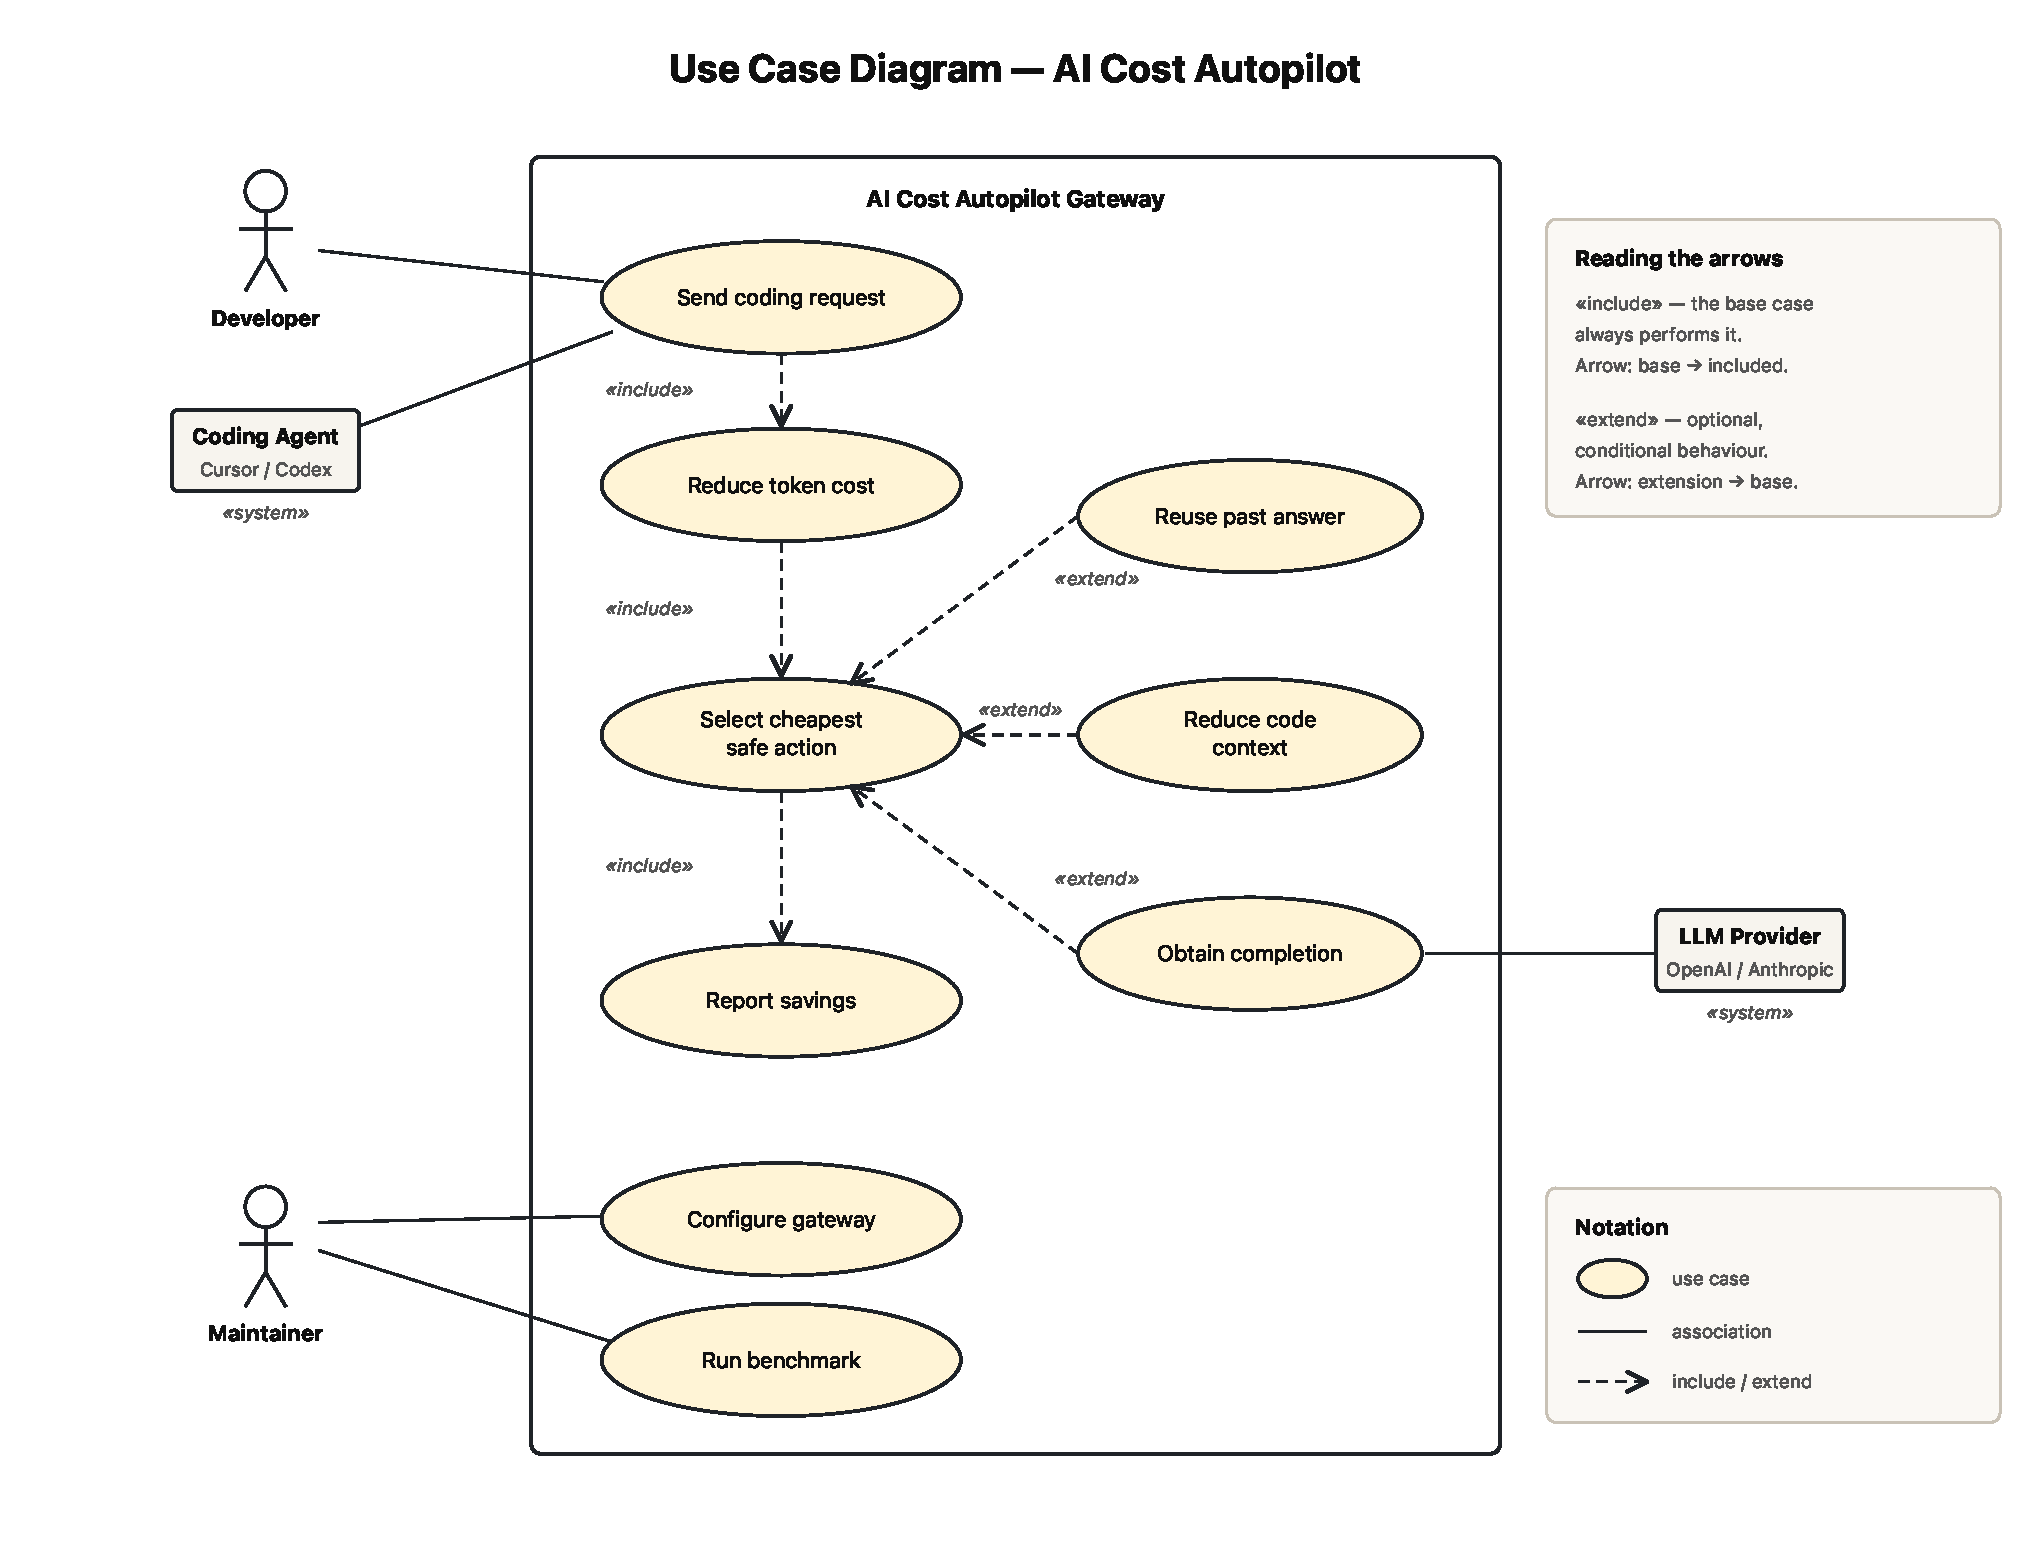
\includegraphics[width=0.95\textwidth, height=0.82\textheight, keepaspectratio]{use-case}
    \caption{Use case diagram.}
    \label{fig:usecase}
\end{figure}

\begin{figure}[H]
    \centering
    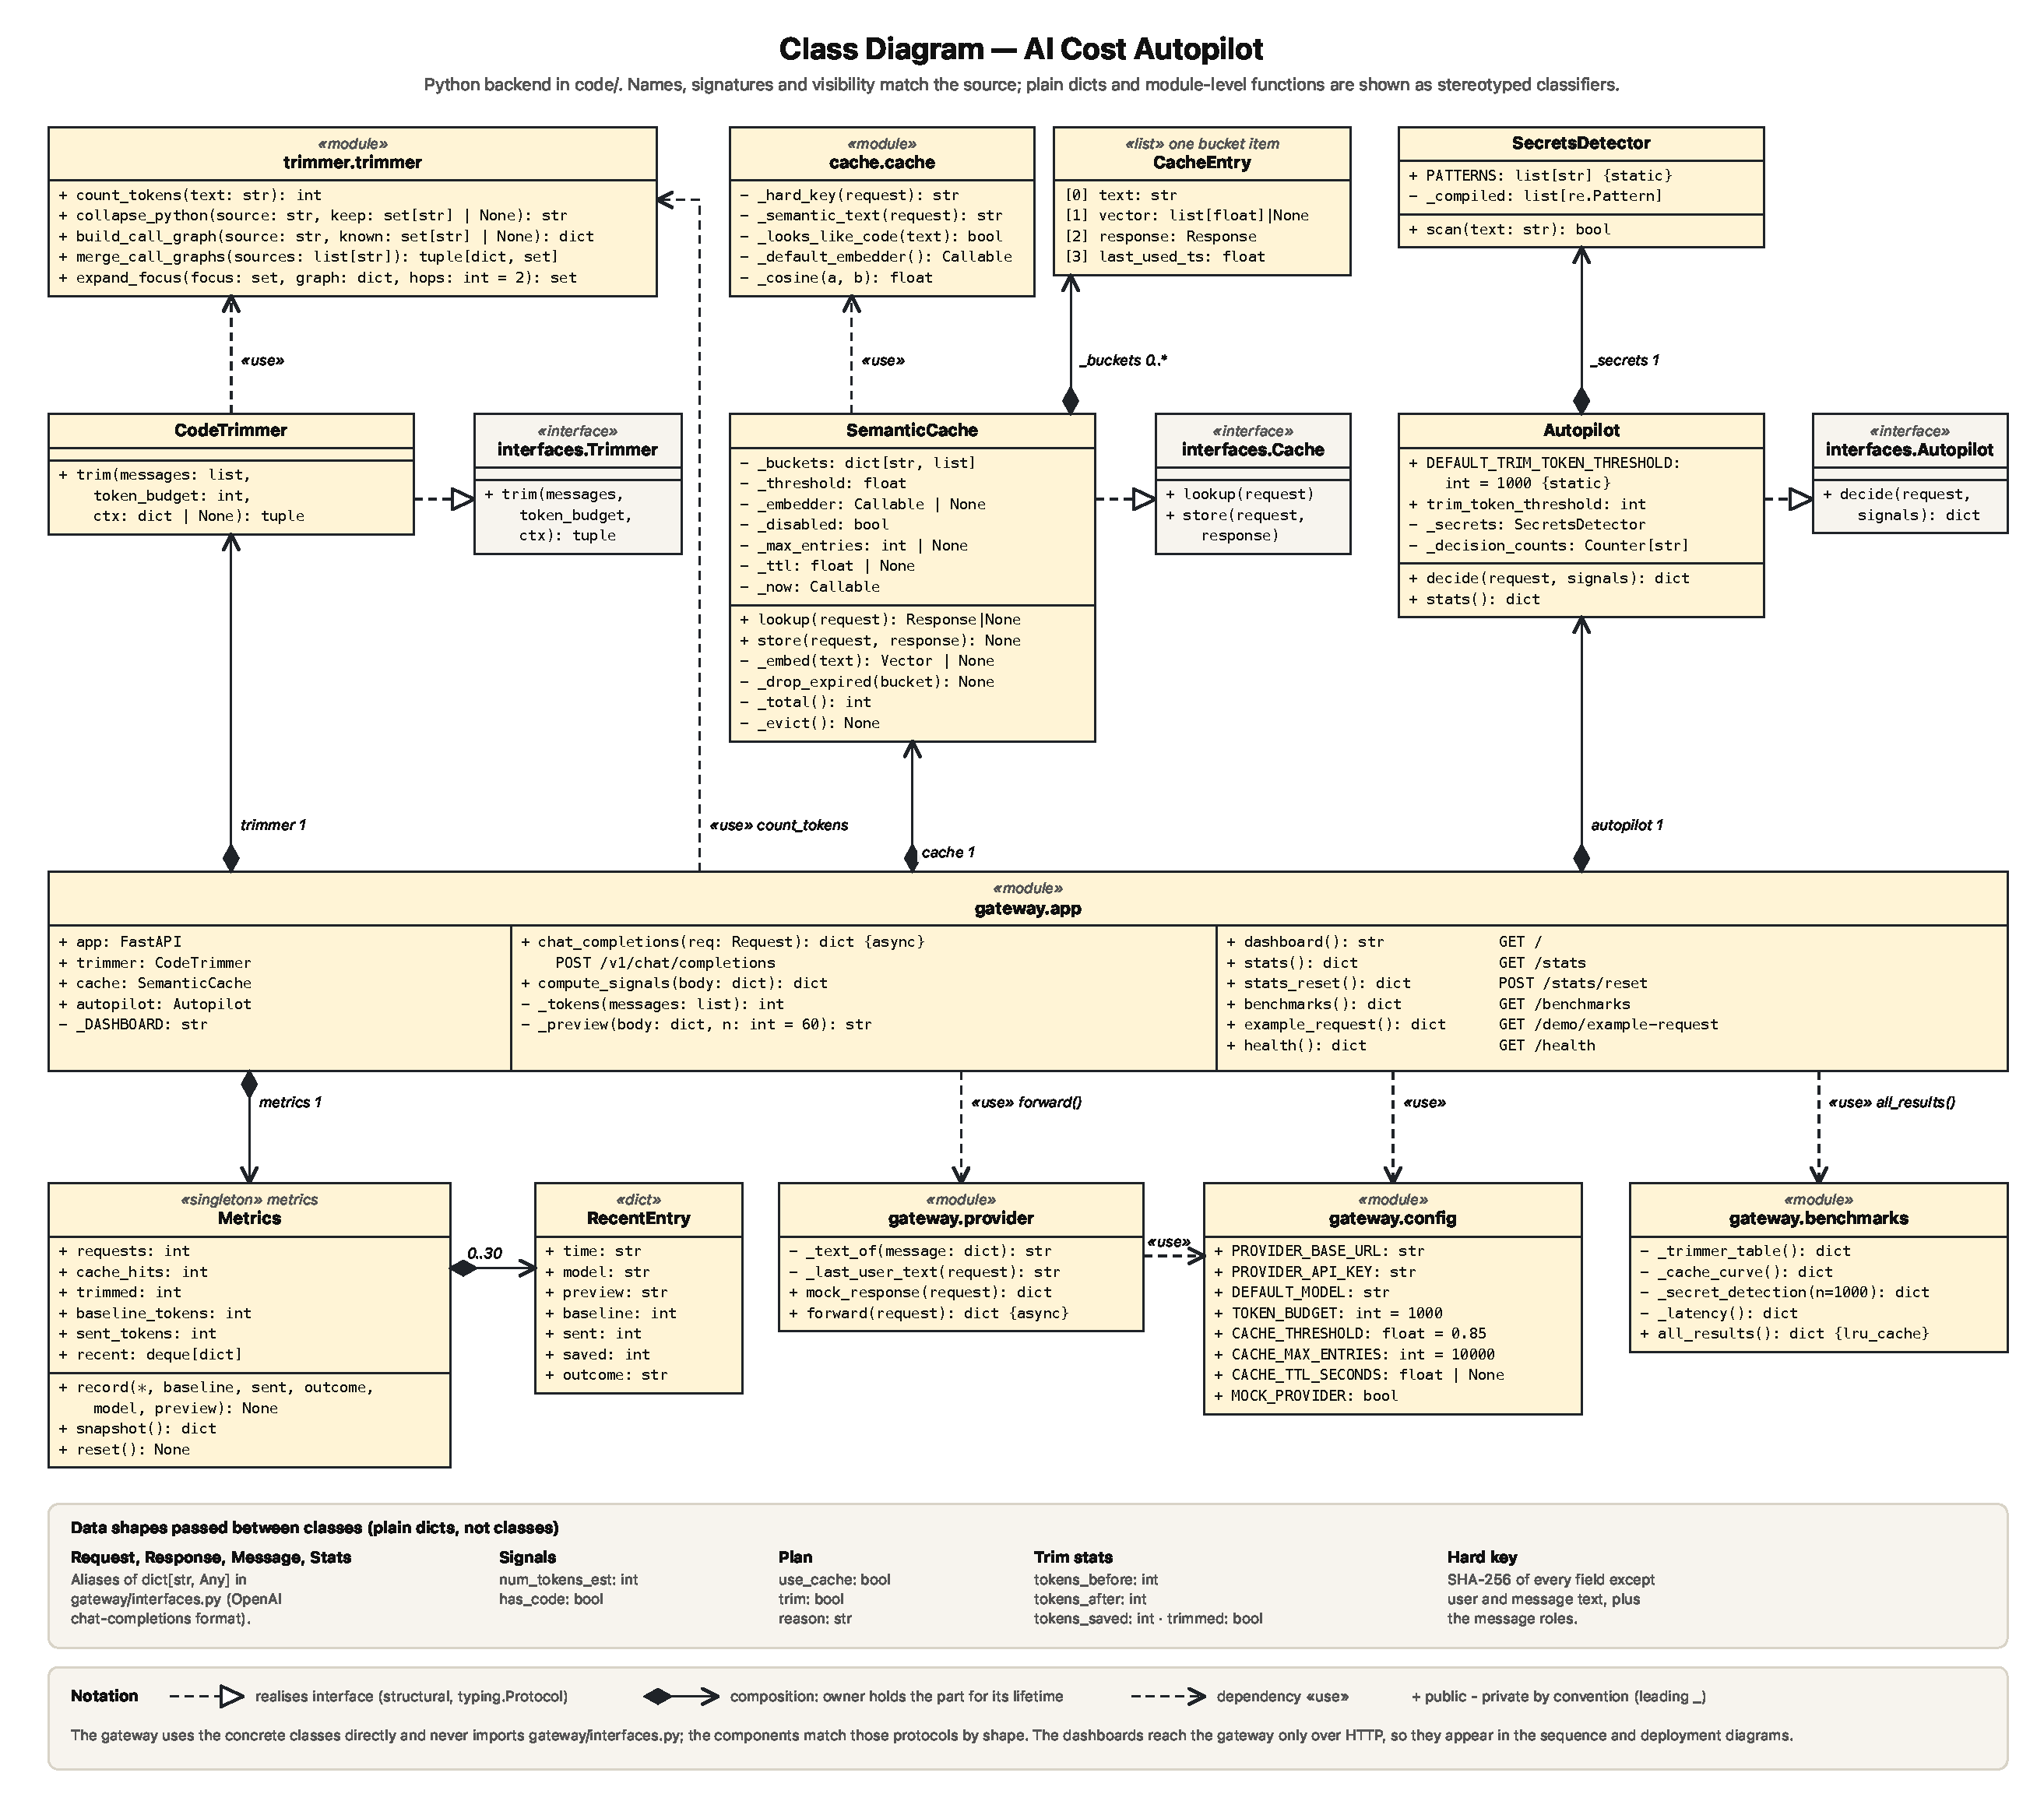
\includegraphics[width=\textwidth, height=0.82\textheight, keepaspectratio]{class-diagram}
    \caption{Class diagram of the gateway and its three components.}
    \label{fig:class}
\end{figure}

\begin{figure}[H]
    \centering
    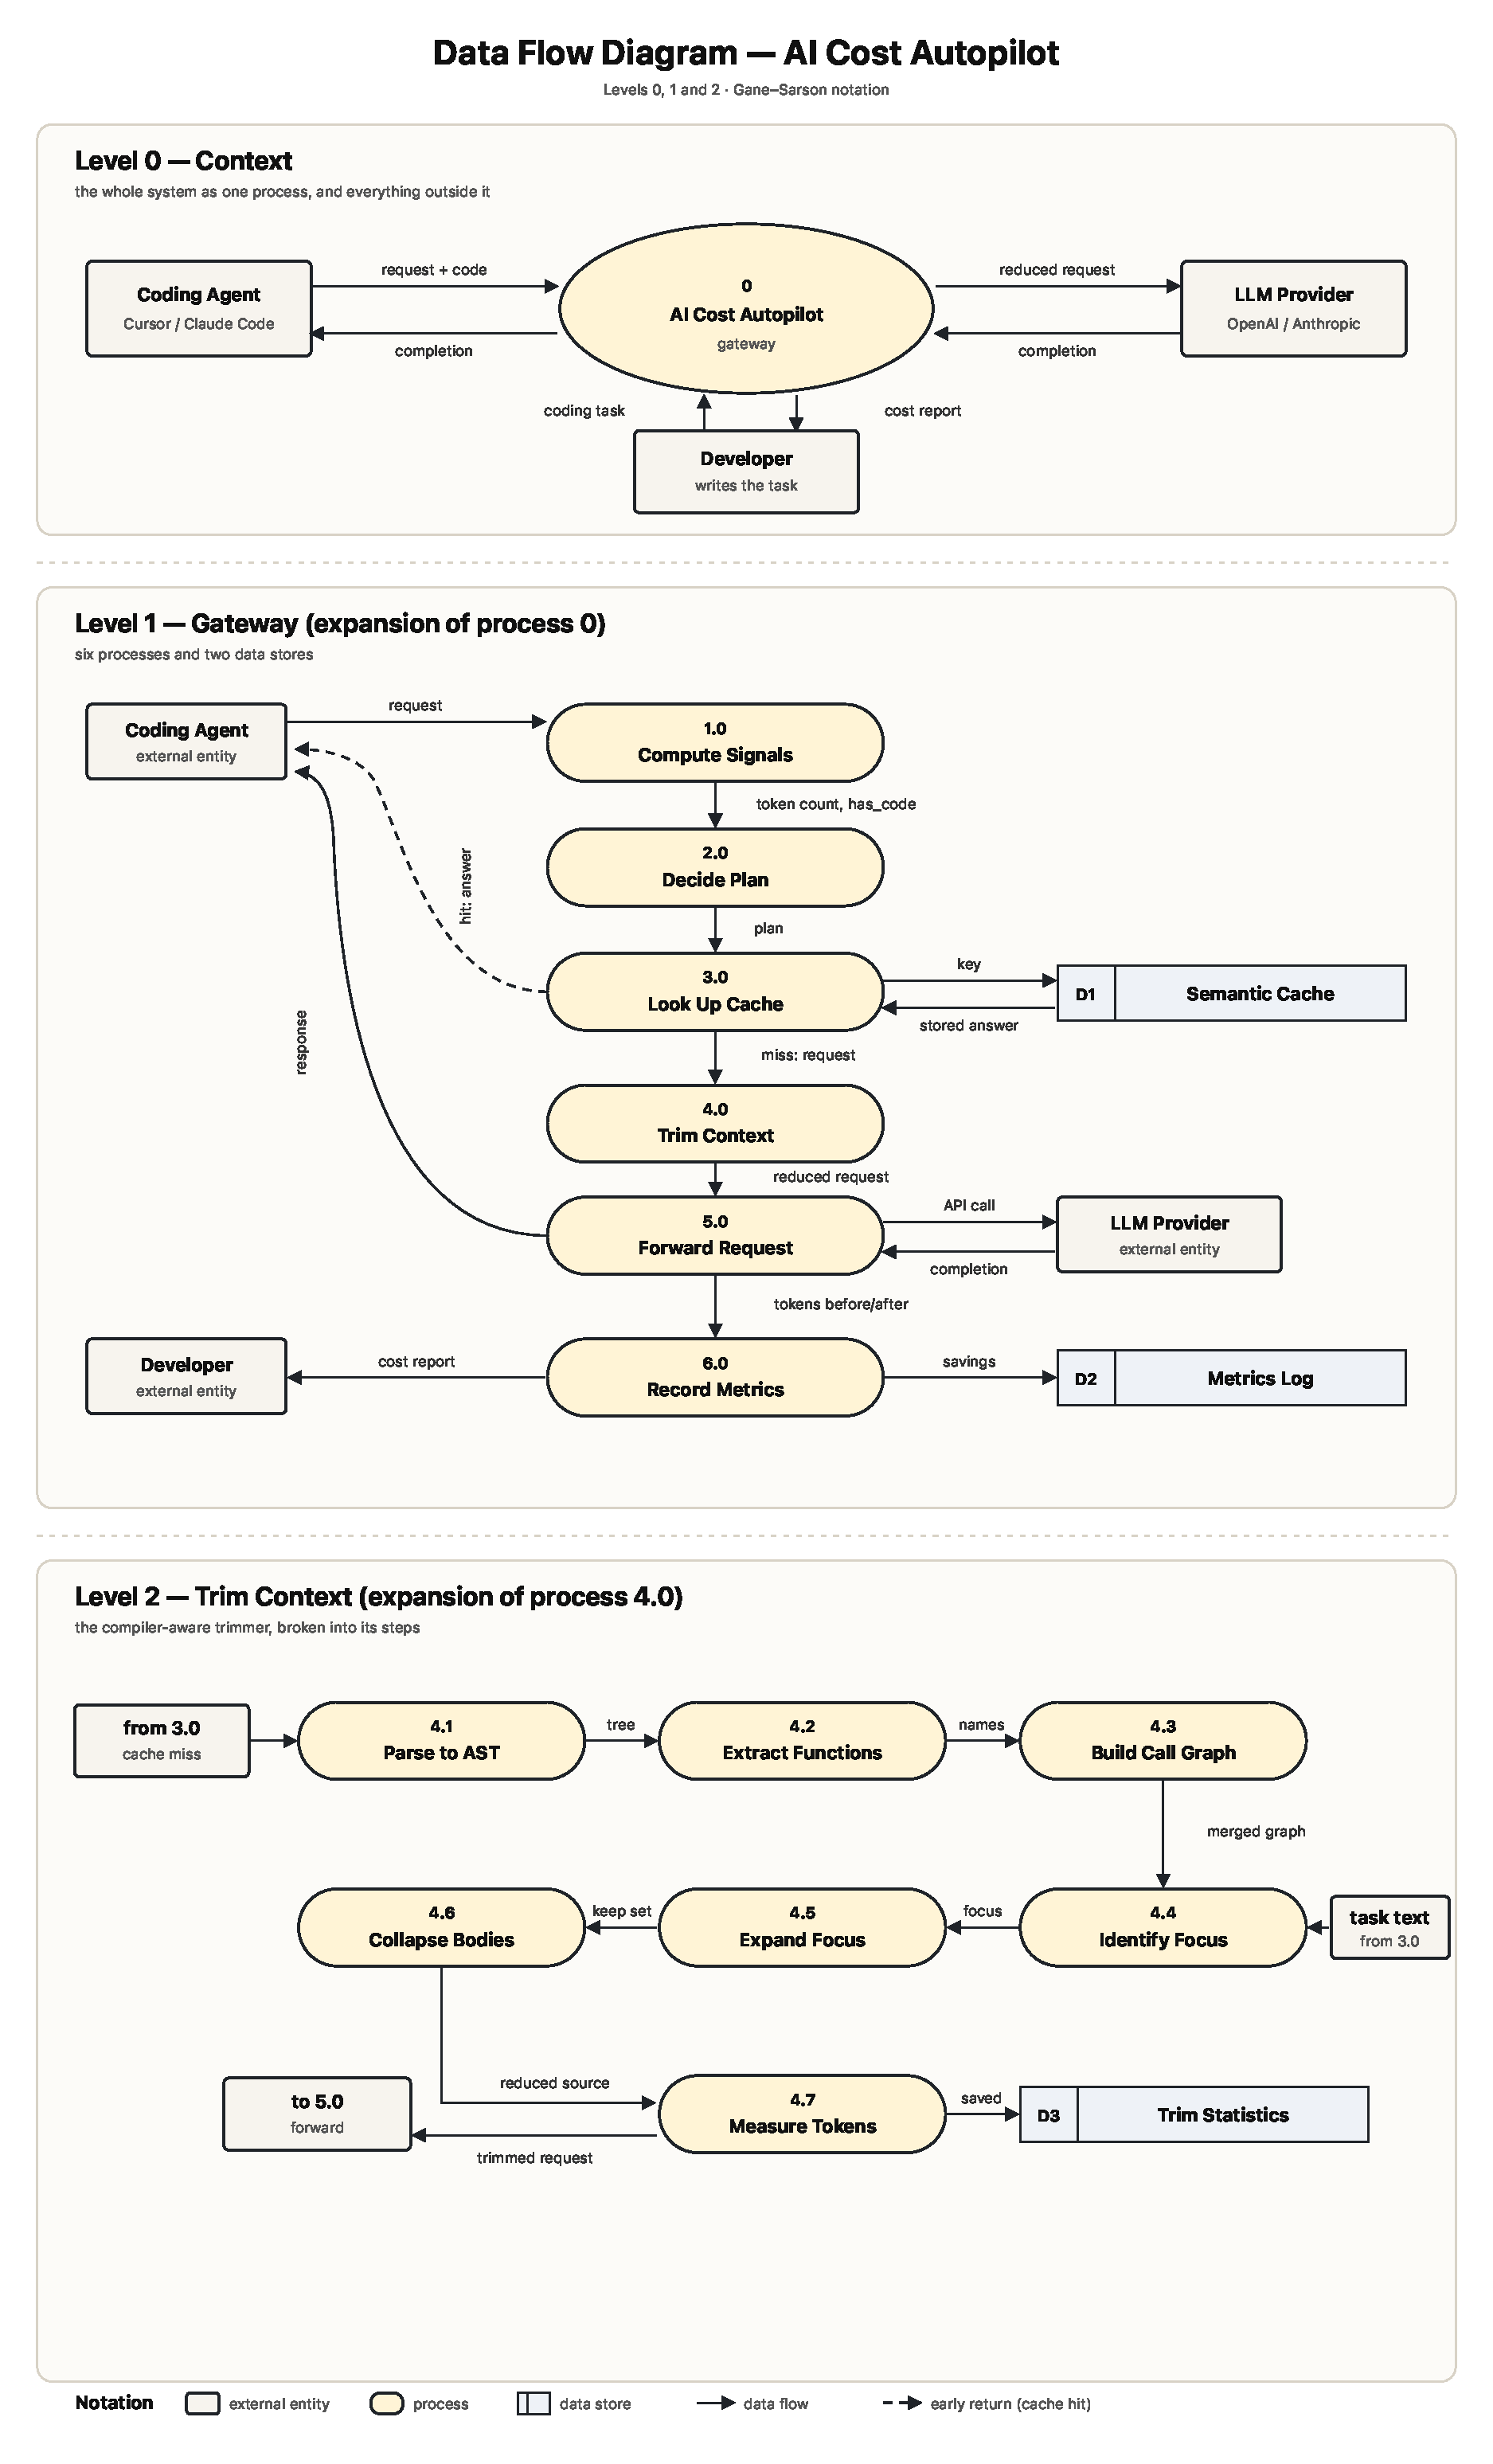
\includegraphics[width=\textwidth, height=0.82\textheight, keepaspectratio]{dfd}
    \caption{Data flow diagram, levels 0, 1 and 2.}
    \label{fig:dfd}
\end{figure}

\begin{figure}[H]
    \centering
    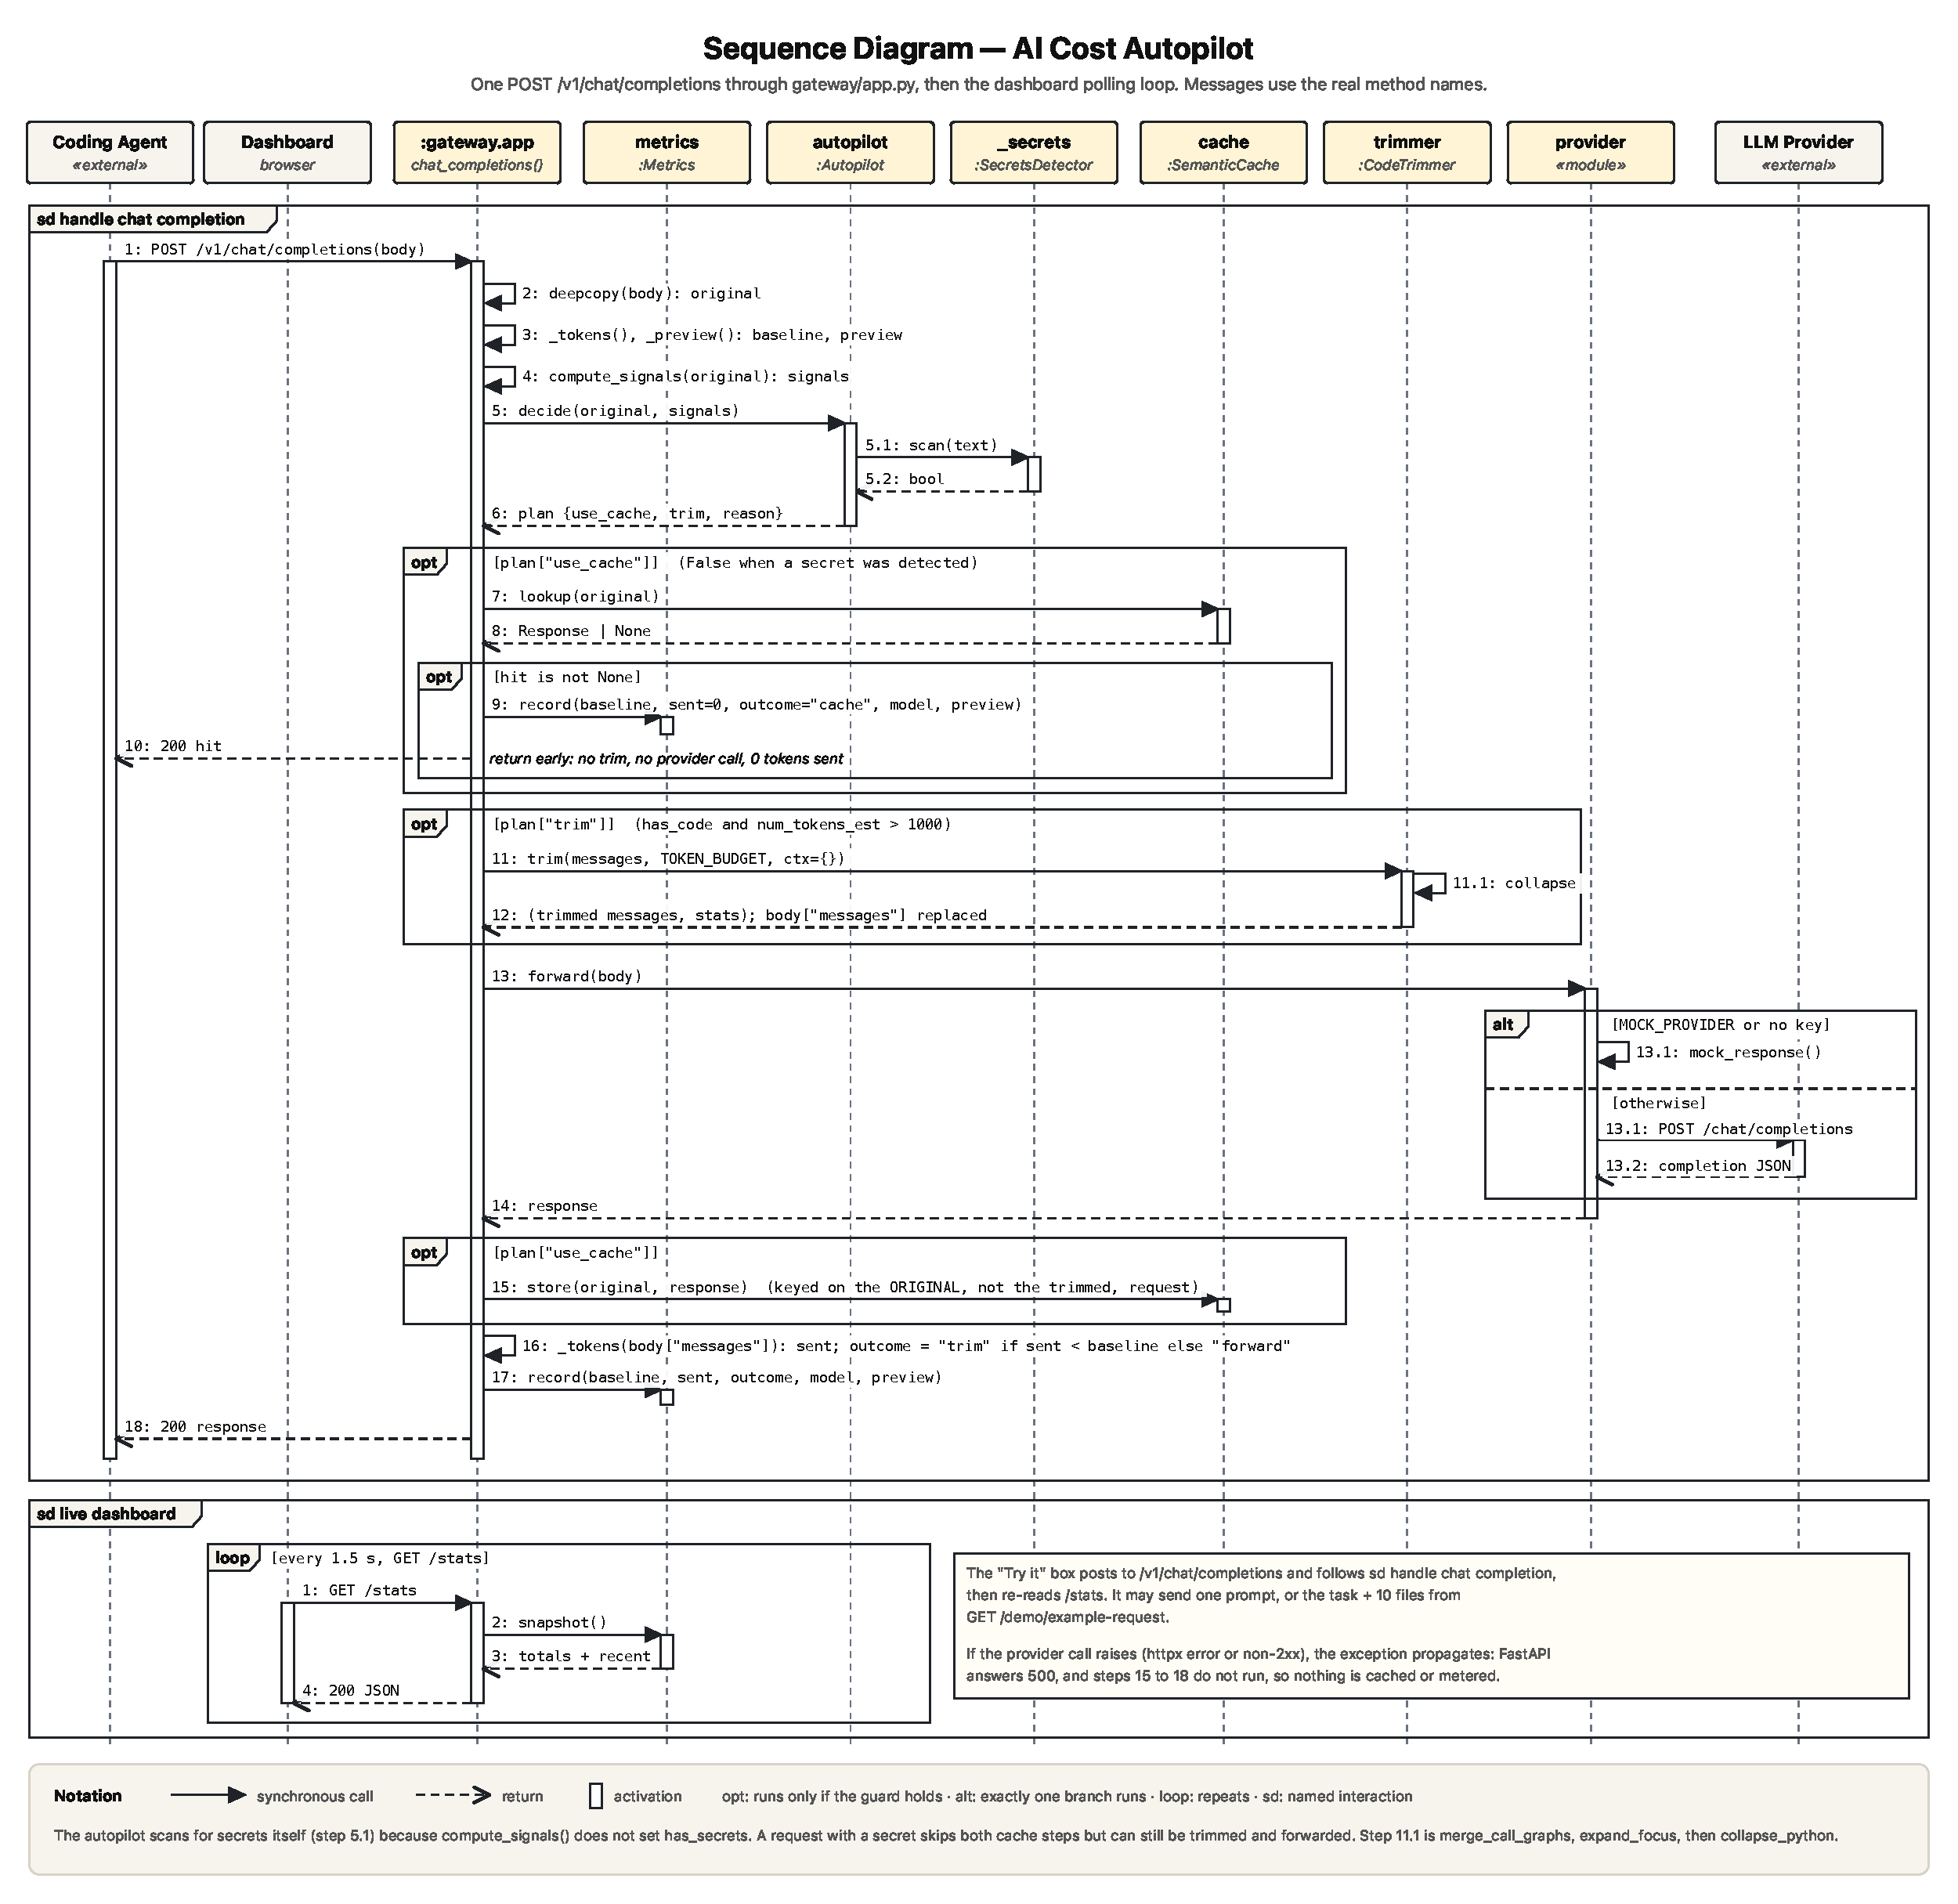
\includegraphics[width=\textwidth, height=0.82\textheight, keepaspectratio]{sequence-diagram}
    \caption{Sequence diagram for one request, including the cache hit path.}
    \label{fig:sequence}
\end{figure}

\begin{figure}[H]
    \centering
    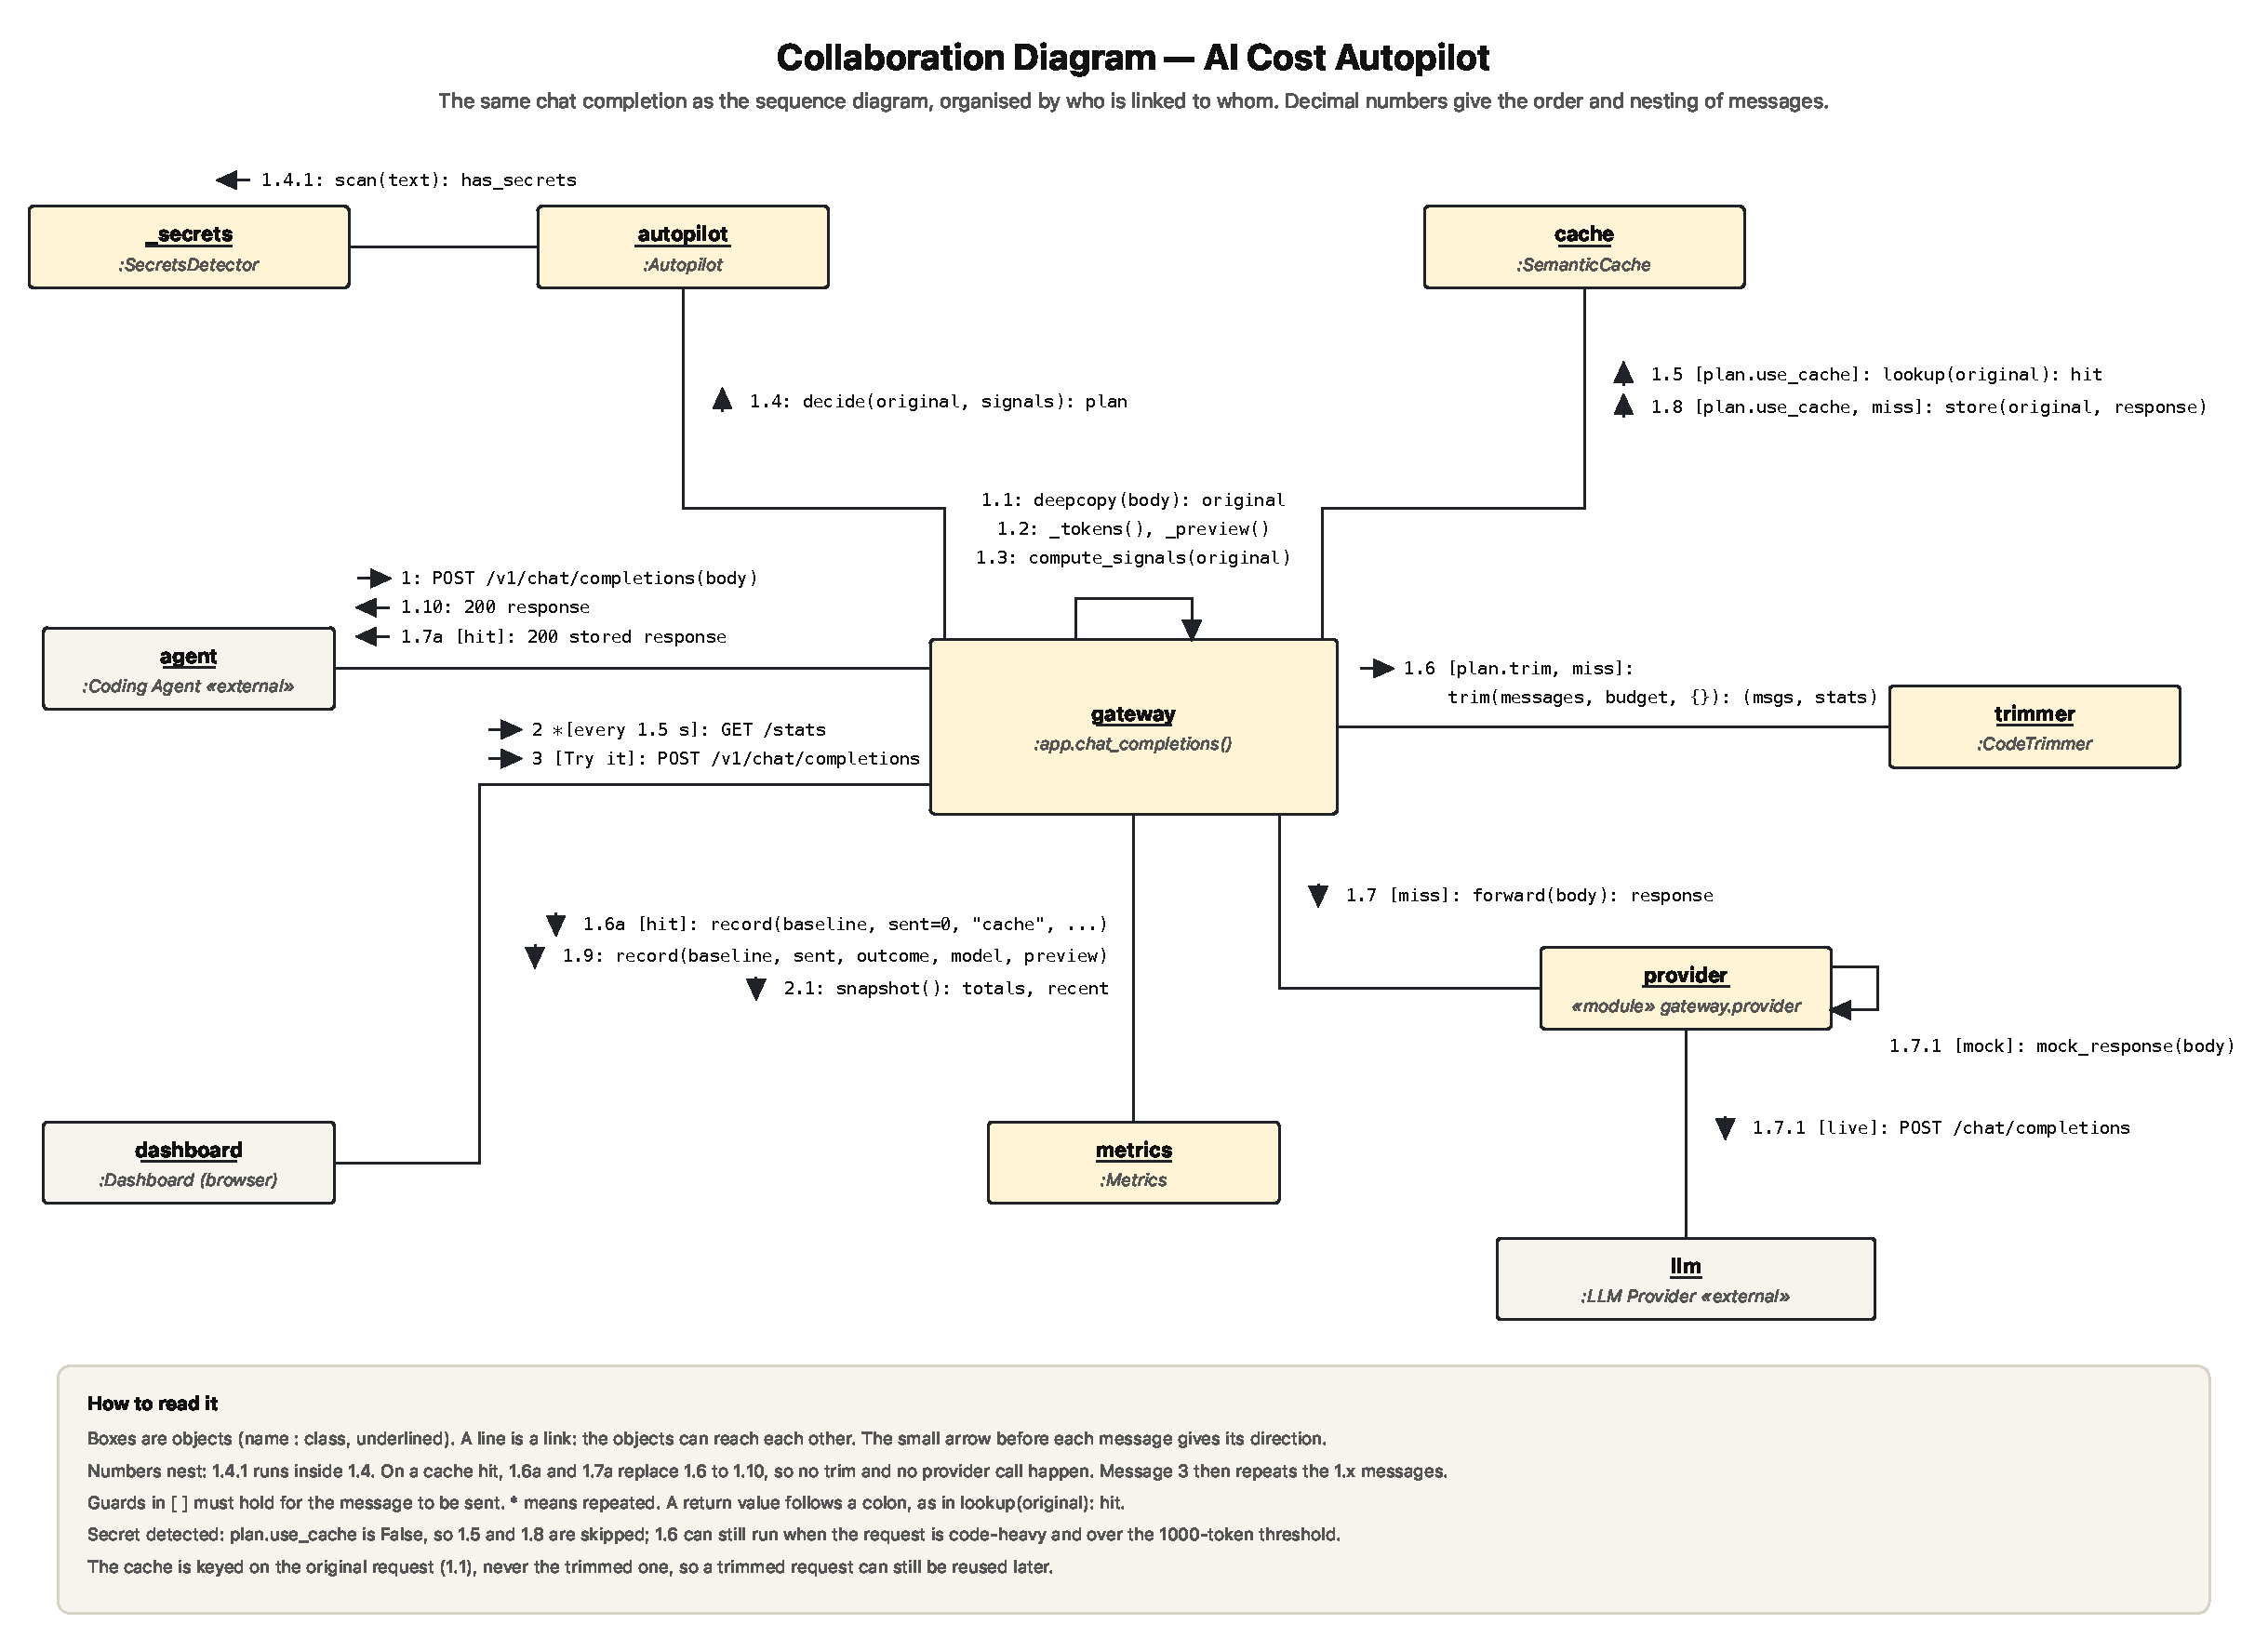
\includegraphics[width=\textwidth, height=0.82\textheight, keepaspectratio]{collaboration-diagram}
    \caption{Collaboration diagram with numbered messages.}
    \label{fig:collaboration}
\end{figure}

\begin{figure}[H]
    \centering
    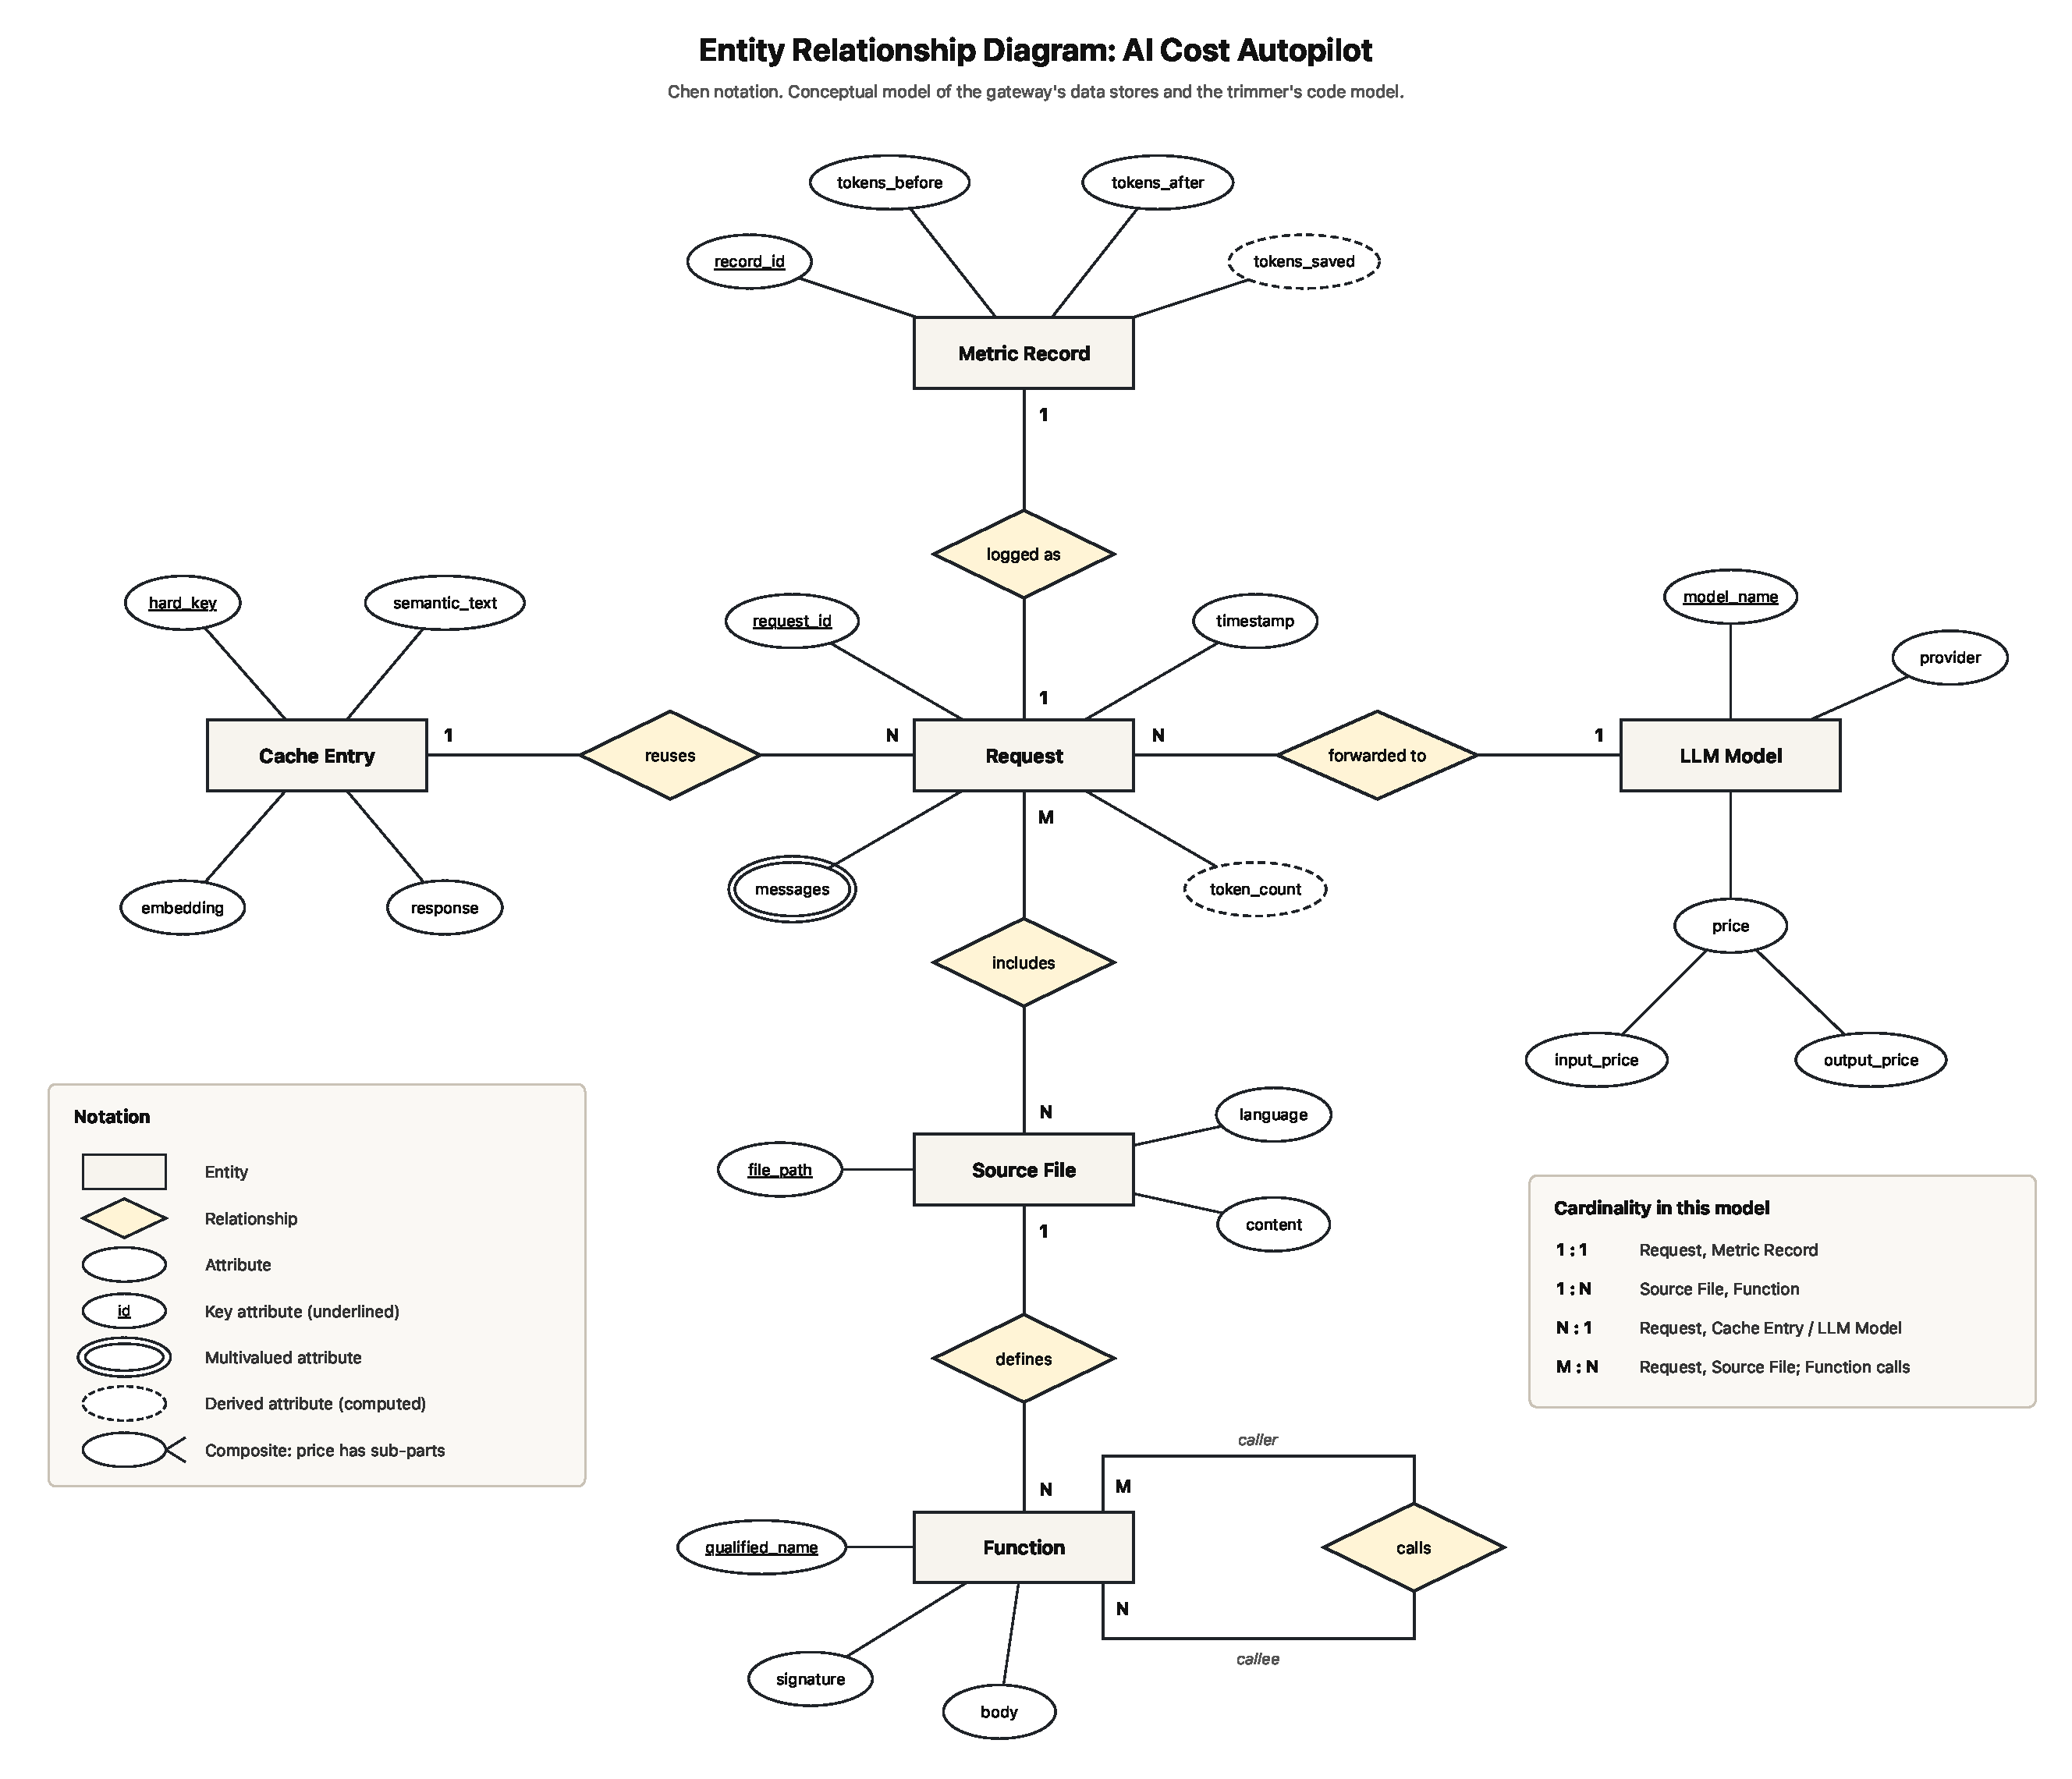
\includegraphics[width=\textwidth, height=0.82\textheight, keepaspectratio]{er}
    \caption{Entity relationship diagram (Chen notation).}
    \label{fig:er}
\end{figure}

\begin{figure}[H]
    \centering
    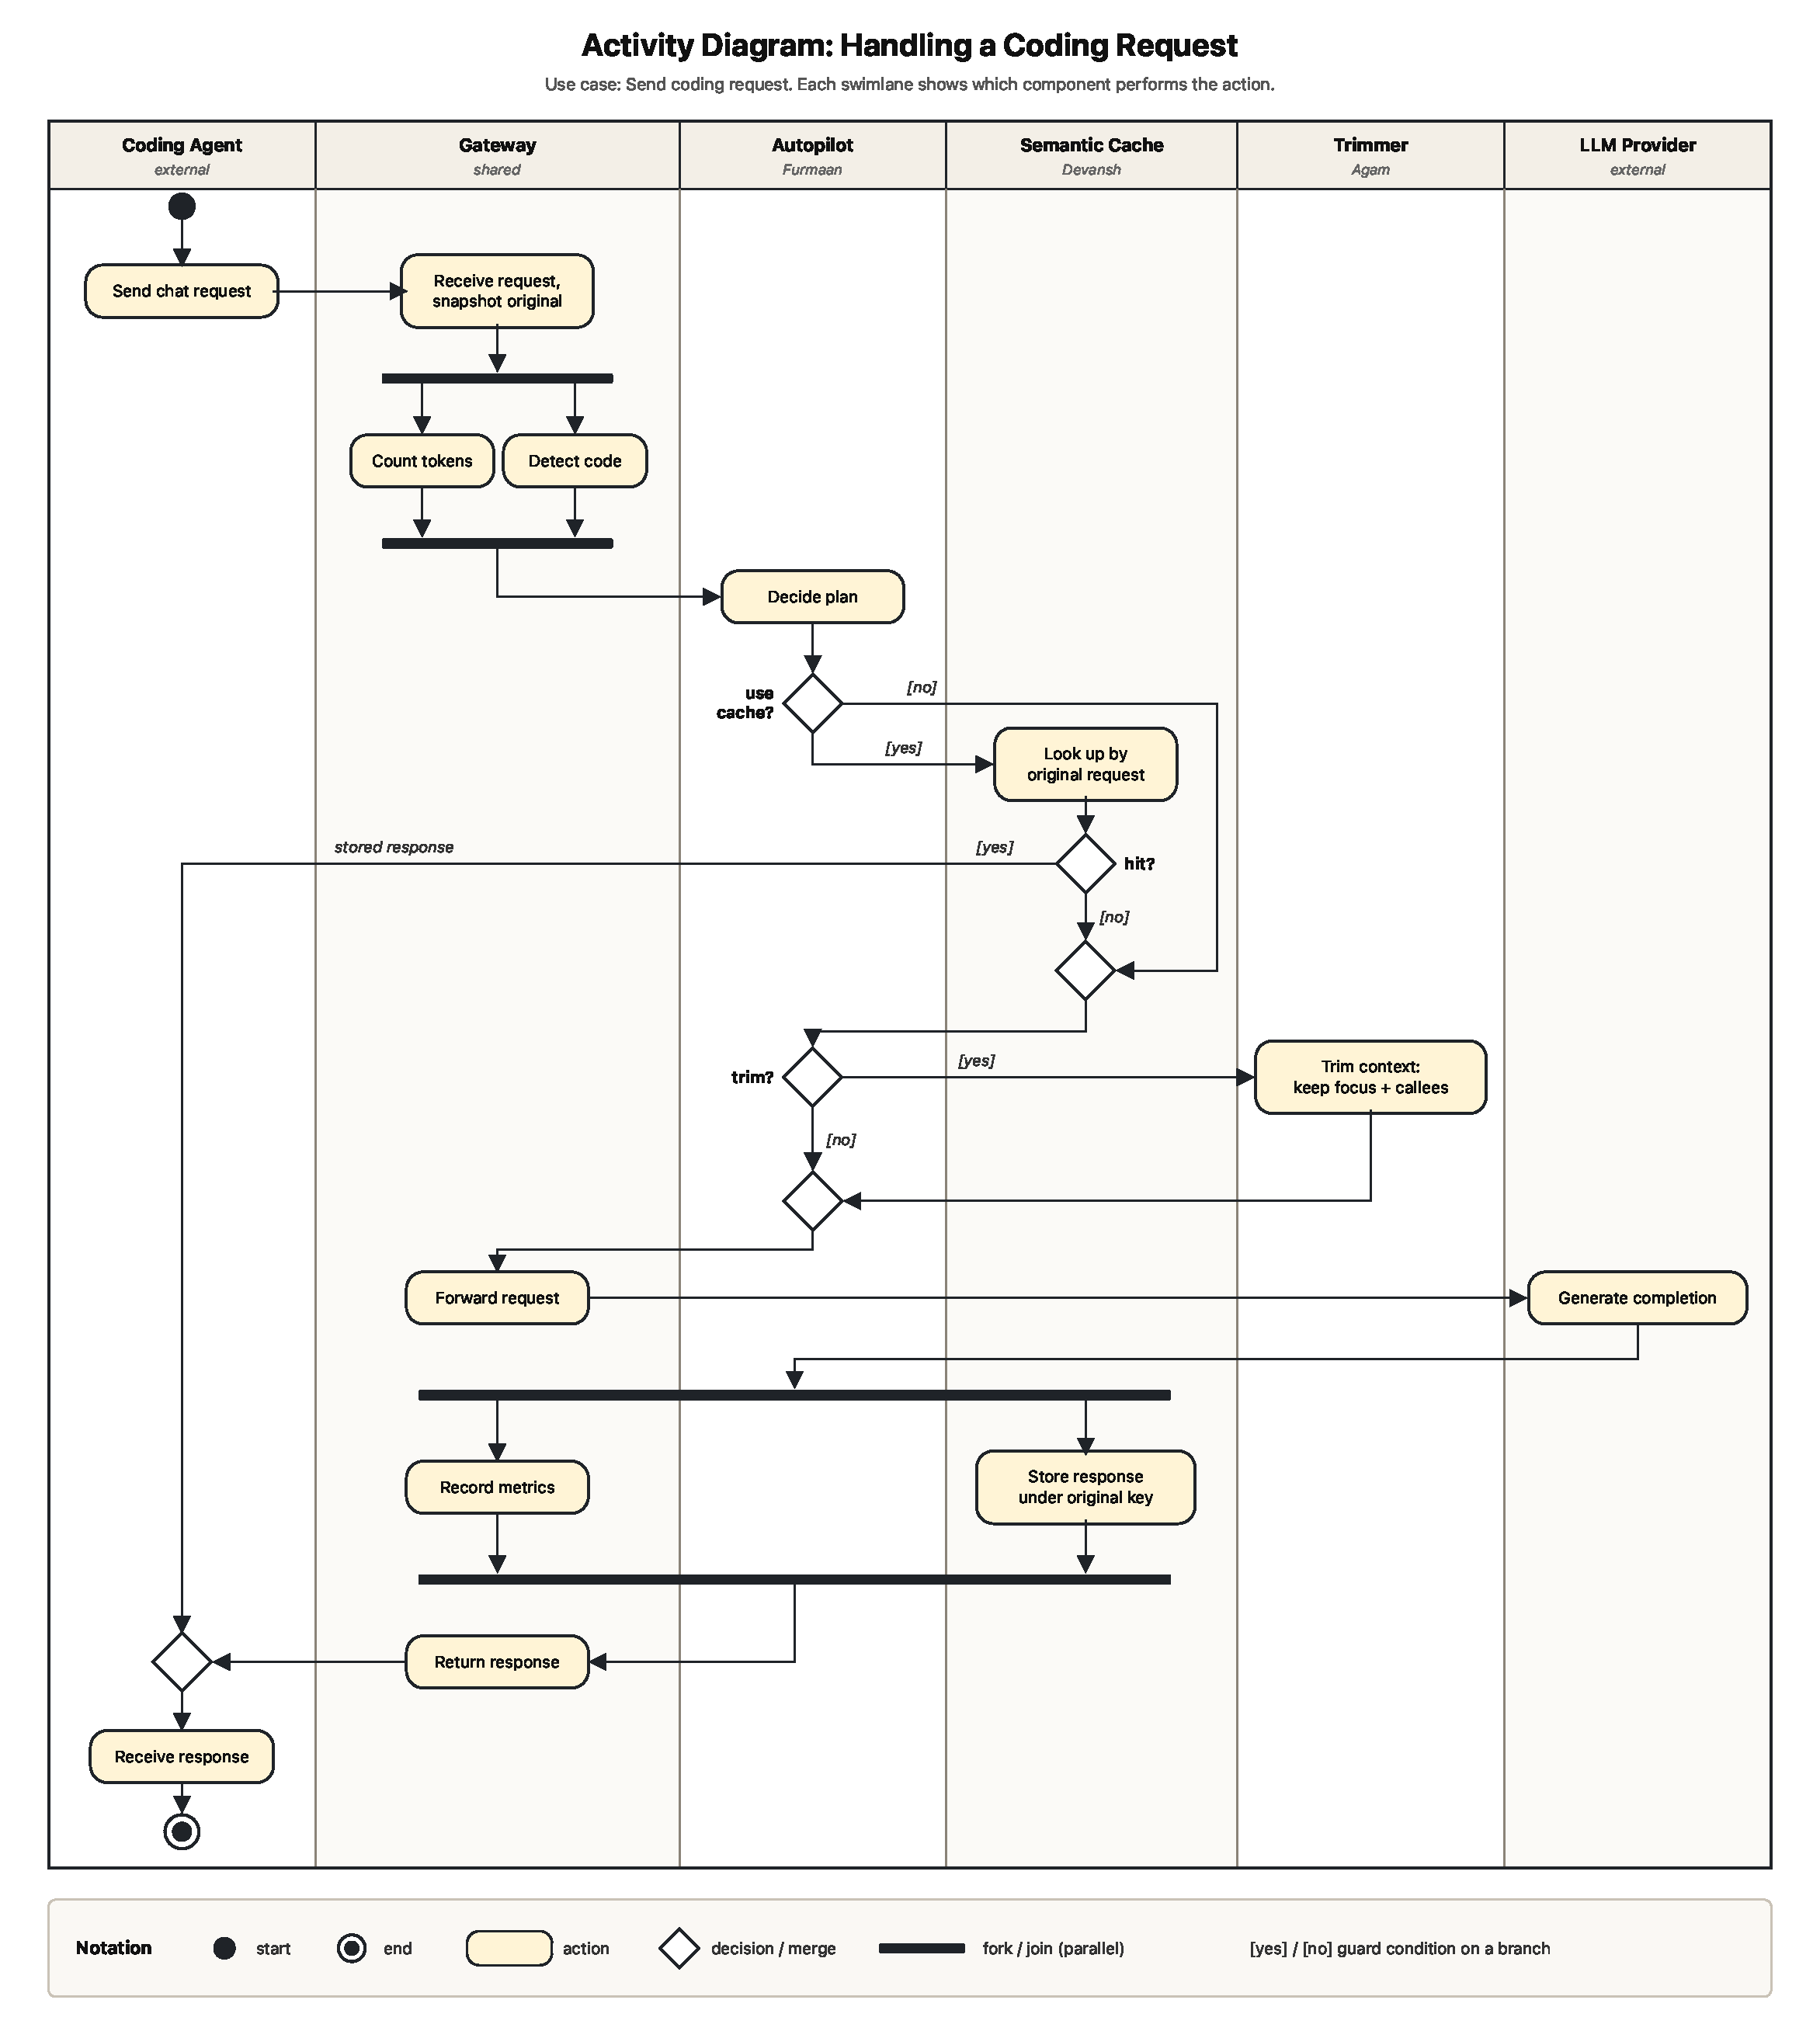
\includegraphics[width=\textwidth, height=0.82\textheight, keepaspectratio]{activity}
    \caption{Activity diagram with swimlanes for handling one coding request.}
    \label{fig:activity}
\end{figure}

\begin{figure}[H]
    \centering
    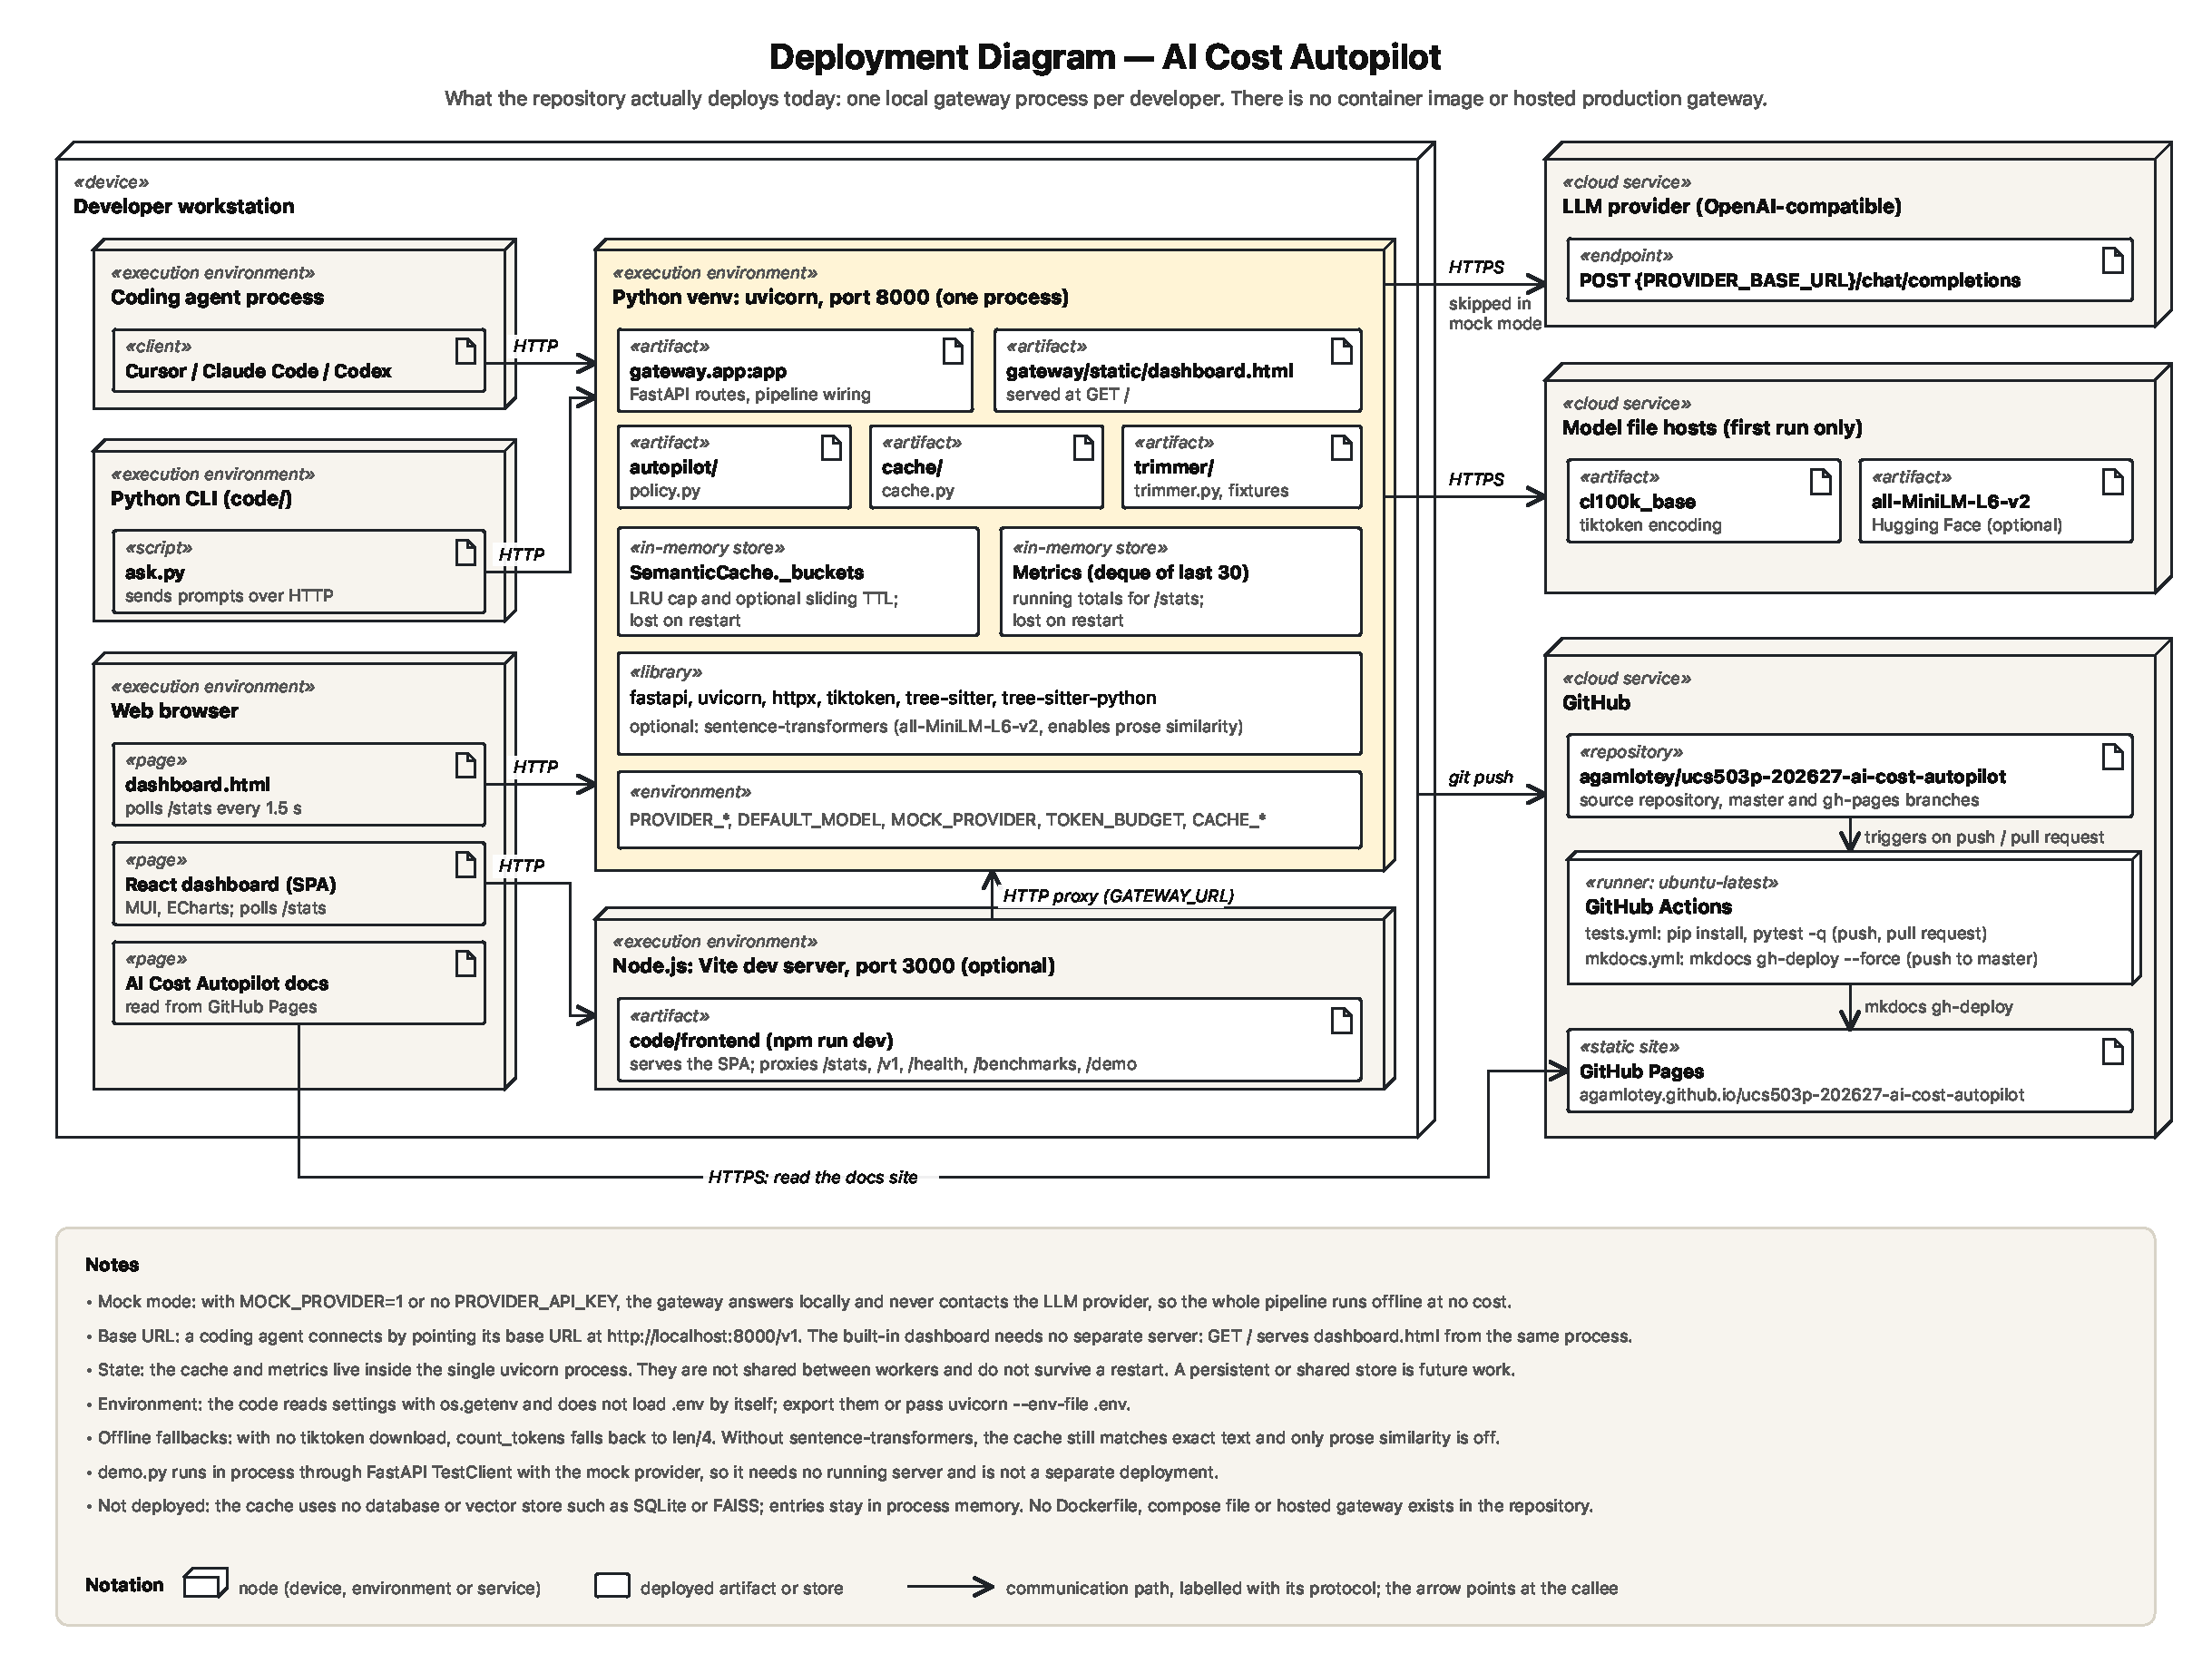
\includegraphics[width=\textwidth, height=0.82\textheight, keepaspectratio]{deployment-diagram}
    \caption{Deployment diagram: where each part of the system runs.}
    \label{fig:deployment}
\end{figure}
